\usetikzlibrary{arrows.meta}
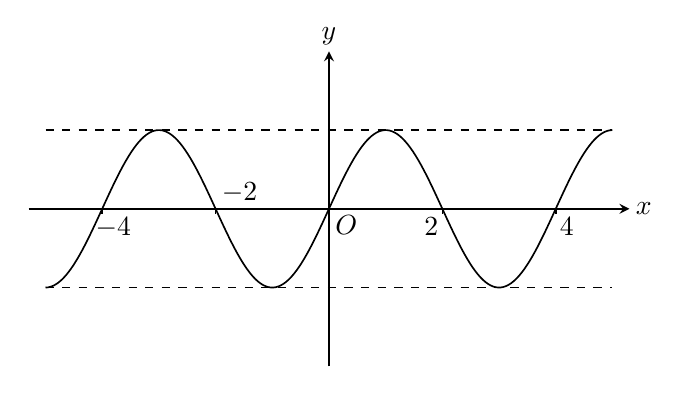
\begin{tikzpicture}[x=0.72cm,y=1.0cm,line width=.6pt,>=stealth,font=\normalsize]
\draw[->] (-5.3,0)--(5.3,0) node[right,inner sep=0pt,xshift=2pt] {$x$};
\draw[->] (0,-2.0)--(0,2.0) node[above,inner sep=0pt,yshift=2pt] {$y$};
\draw (-4,0)--(-4,-0.07);
\draw (-2,0)--(-2,-0.07);
\draw (2,0)--(2,-0.07);
\draw (4,0)--(4,-0.07);
\node[below,inner sep=0pt,xshift=4pt,yshift=-3pt] at (-4,0) {$-4$};
\node[above right,inner sep=0pt,xshift=2pt,yshift=2pt] at (-2,0) {$-2$};
\node[below,inner sep=0pt,xshift=-4pt,yshift=-3pt] at (2,0) {$2$};
\node[below,inner sep=0pt,xshift=4pt,yshift=-3pt] at (4,0) {$4$};
\node[below right,inner sep=0pt,xshift=2pt,yshift=-2pt] at (0,0) {$O$};
\draw[dashed] (-5.0,1)--(5.0,1);
\draw[dashed] (-5.0,-1)--(5.0,-1);
\draw[domain=-5.0:5.0,samples=220] plot (\x,{sin(deg(pi*\x/2))});
\end{tikzpicture}
